\subsection{How is tolerance measured?}
\label{measurement:tolerance}

Tolerance was measured with four Likert items (1--5 scale), following the
original Wildlife Tolerance Model questionnaire design \citep{Kansky2016}:

\begin{itemize}
  \item \emph{Tol1}: support for non-lethal management strategies (e.g.\
    relocation, fencing) -- positively framed.
  \item \emph{Tol2}: agreement that the government should take stricter
    measures to control the wild boar population -- reverse-coded, so that a
    higher raw score corresponds to lower tolerance.
  \item \emph{Tol3}: perceived threat to personal safety from wild boars --
    reverse-coded.
  \item \emph{Tol4}: willingness to accept some damage caused by wild boars --
    positively framed.
\end{itemize}

After reverse-coding, all four items are oriented so that 1 indicates low
tolerance and 5 indicates high tolerance. Conceptually the four items are not
interchangeable: they capture management preferences, policy attitudes, fear,
and damage acceptance separately, which is one reason the original model
treats tolerance as a multidimensional construct rather than a single
attitude.

\subsection{Exploratory and confirmatory checks rule out one item}
\label{measurement:efa-cfa}

Before any structural model was fit, we checked whether the four tolerance
items actually behave as a single, internally consistent scale, using three
independent methods of increasing formality.

First, a simple reliability check. For a $k$-item scale with item variances
$\sigma_i^2$ and total-score variance $\sigma_X^2$ (the variance of the
row-wise item sum $X = \sum_i \text{item}_i$), Cronbach's alpha is

\begin{equation}
\alpha = \frac{k}{k-1}\left(1 - \frac{\sum_{i=1}^{k}\sigma_i^2}{\sigma_X^2}\right).
\label{eq:alpha}
\end{equation}

Equivalently, in terms of the average pairwise inter-item correlation
$\bar{r}$, $\alpha = k\bar{r} / (1 + (k-1)\bar{r})$: a scale whose items
correlate strongly with each other has a total-score variance much larger
than the sum of the individual item variances, and $\alpha$ close to 1; a
scale whose items are unrelated has $\alpha$ close to 0. The original
four-item tolerance scale has low internal consistency by this measure
(Cronbach's $\alpha = 0.34$, well below the conventional 0.70 threshold for
a reliable scale), and Tol3's item-rest correlation (its correlation
with the sum of the other three items) is $-0.004$ -- essentially
unrelated to the rest of the scale. Second, exploratory factor analysis
(EFA; R package \texttt{psych} \citep{Rpsych}, with rotations from
\texttt{GPArotation} \citep{RGPArotation}) agrees:
Tol3's loading on a single factor is $-0.009$, close to zero. Third, confirmatory factor
analysis (CFA; R packages \texttt{lavaan} \citep{Rlavaan} and
\texttt{semTools} \citep{RsemTools}, WLSMV estimator for ordinal
indicators) confirms this independently, in a formal one-factor model with a
significance test per item: Tol3's standardised loading is 0.006 with
$p = .896$, statistically indistinguishable from zero, while Tol1, Tol2, and
Tol4 all load significantly (Table~\ref{tab:tol3}).

One feature of this confirmatory model must be disclosed. The standardised
loading of Tol2 is 1.04, which is larger than 1 and implies a negative
residual variance ($-0.09$) for that item: an improper solution, known as a
Heywood case. It arises because the factor is defined almost entirely by
the one strong correlation in the block, between Tol1 and Tol2 (polychoric
$r = 0.51$), while Tol4 relates only moderately to Tol2 ($0.37$) and weakly
to Tol1 ($0.17$). The individual loadings in Table~\ref{tab:tol3} should
therefore not be over-interpreted. The conclusion about Tol3 does not
depend on it: in a proper solution, obtained by constraining the Tol1 and
Tol2 loadings to be equal, Tol3 still loads at $0.03$ ($p = .50$), and with
a robust maximum-likelihood estimator that treats the items as continuous it
loads at $-0.01$ ($p = .78$). The improper solution is, however, further
evidence that tolerance is a weak scale, dominated by two items, and this is
a limitation of every result that uses it.

Three methods that make different assumptions -- a bivariate correlation, an
exploratory factor model, and a confirmatory factor model with a formal
hypothesis test -- independently agree that Tol3 does not belong with the
other three tolerance items. Table~\ref{tab:tol3} reports the
full item-level detail behind this conclusion.

\begin{table}[htbp]
\centering
\caption{Item-level reliability and confirmatory factor analysis (CFA)
results for the four original tolerance items. Item-rest $r$ is each item's
correlation with the sum of the other three (n=625). CFA loading is the
standardised factor loading from a single-factor confirmatory model on all
four items (lavaan, WLSMV estimator, ordinal indicators).}
\label{tab:tol3}
\begin{tabular}{lp{4.3cm}rrrr}
\hline
\textbf{Item} & \textbf{Statement} & \textbf{Item-rest $r$} & \textbf{CFA loading} & \textbf{$z$} & \textbf{$p$} \\
\hline
Tol1 & Supports non-lethal management & 0.324 & 0.49 & (ref.) & --- \\
Tol2 & Govt should not crack down (rev.) & 0.387 & 1.04 & 4.79 & $<.001$ \\
Tol3 & Perceived personal-safety threat (rev.) & $-0.004$ & 0.006 & 0.13 & .896 \\
Tol4 & Accepts some damage & 0.150 & 0.35 & 9.20 & $<.001$ \\
\hline
\end{tabular}
\end{table}

\begin{figure}[htbp]
\centering
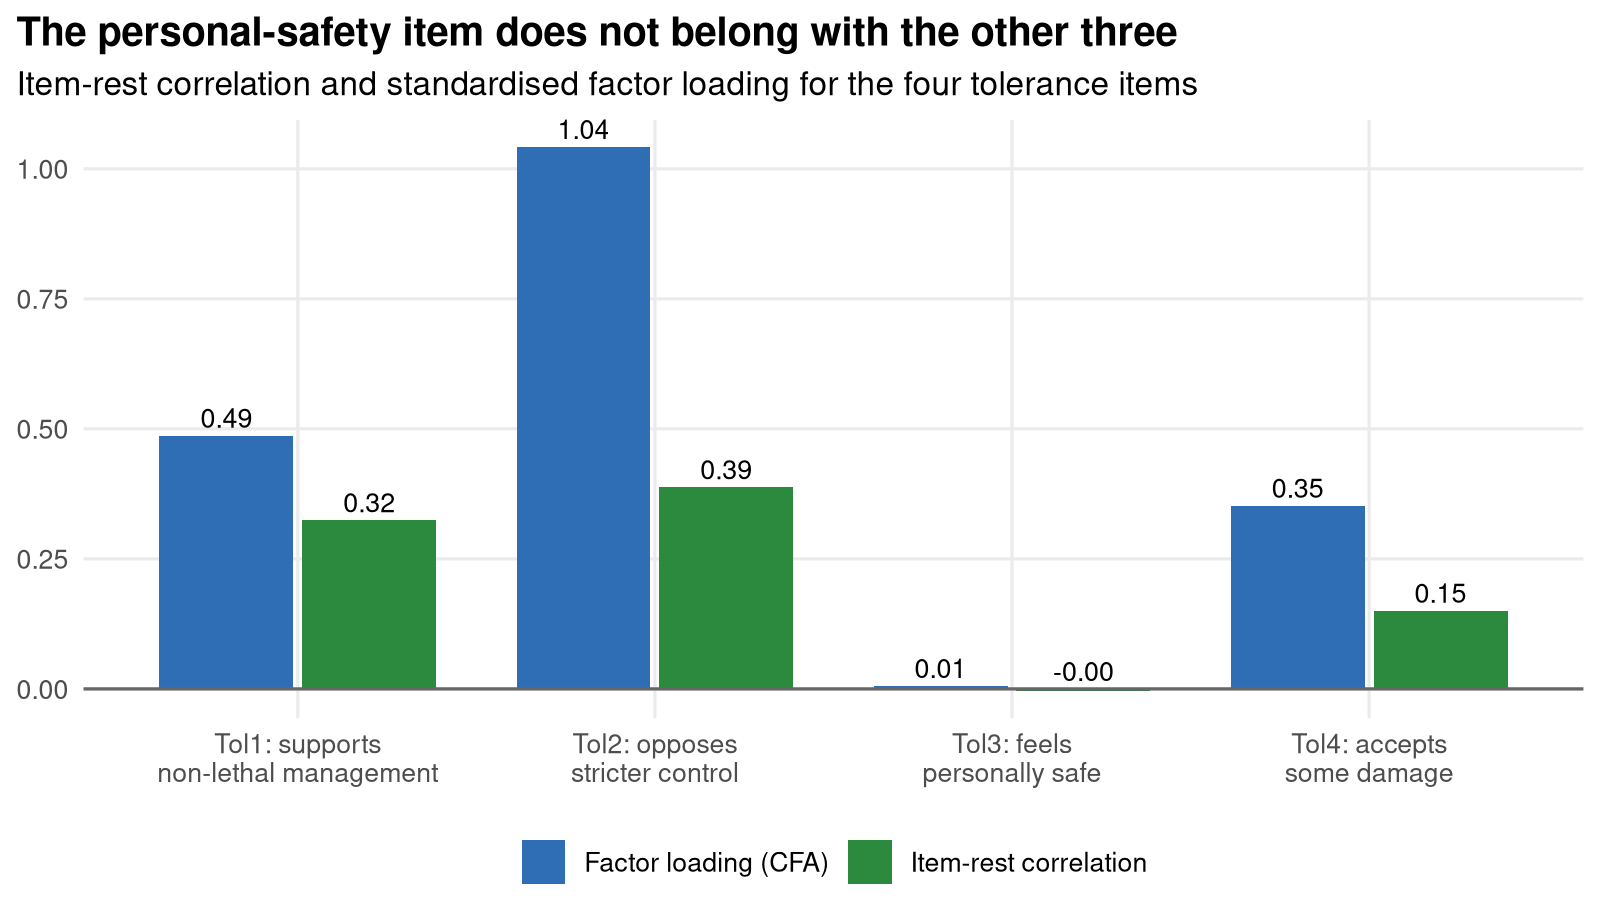
\includegraphics[width=0.85\textwidth]{figures/fig_tol_items.png}
\caption{Item-rest correlation and standardised CFA loading by tolerance
item. Tol3 is indistinguishable from zero on both measures. The Tol2 loading
above 1 is the improper solution discussed in the text.}
\label{fig:tol-items}
\end{figure}

Figure~\ref{fig:tol-items} shows the same pattern graphically: Tol3's bars
are flat on the floor on both measures, while the other three items are
clearly elevated. On this basis we defined the primary tolerance
construct as the three-item composite Tol1+Tol2+Tol4, and kept the original
four-item version only as a named robustness variant. Dropping Tol3 raises
reliability from $\alpha = 0.34$ to $\alpha = 0.50$ (ordinal $\alpha = 0.62$,
computed from polychoric rather than Pearson item correlations, which better
suit five-category ordinal data); every downstream structural path reported
in Section~\ref{model} is materially unchanged between the three-item and
four-item specifications. We also computed the reliability and validity
statistics that a reflective PLS-SEM construct is usually expected to report:
for the three-item tolerance scale, composite reliability is 0.781 and
average variance extracted (AVE) is 0.551, both above their conventional
0.70 and 0.50 thresholds respectively, even though Cronbach's $\alpha$
(0.577 as reported by the PLS-SEM software, which standardises the items;
0.50 on the raw items) and $\rho_A$ (0.620) remain below 0.70. This split is expected for a short, unevenly-loading three-item
composite (Tol2 loads far more strongly than Tol4) and is a known limitation
of $\alpha$ and $\rho_A$ for such scales, not a contradiction of the CFA
result above. Figure~\ref{fig:reliability} shows the progression from the
original four-item raw alpha through the two three-item variants, alongside
the conventional 0.70 threshold.

\begin{figure}[htbp]
\centering
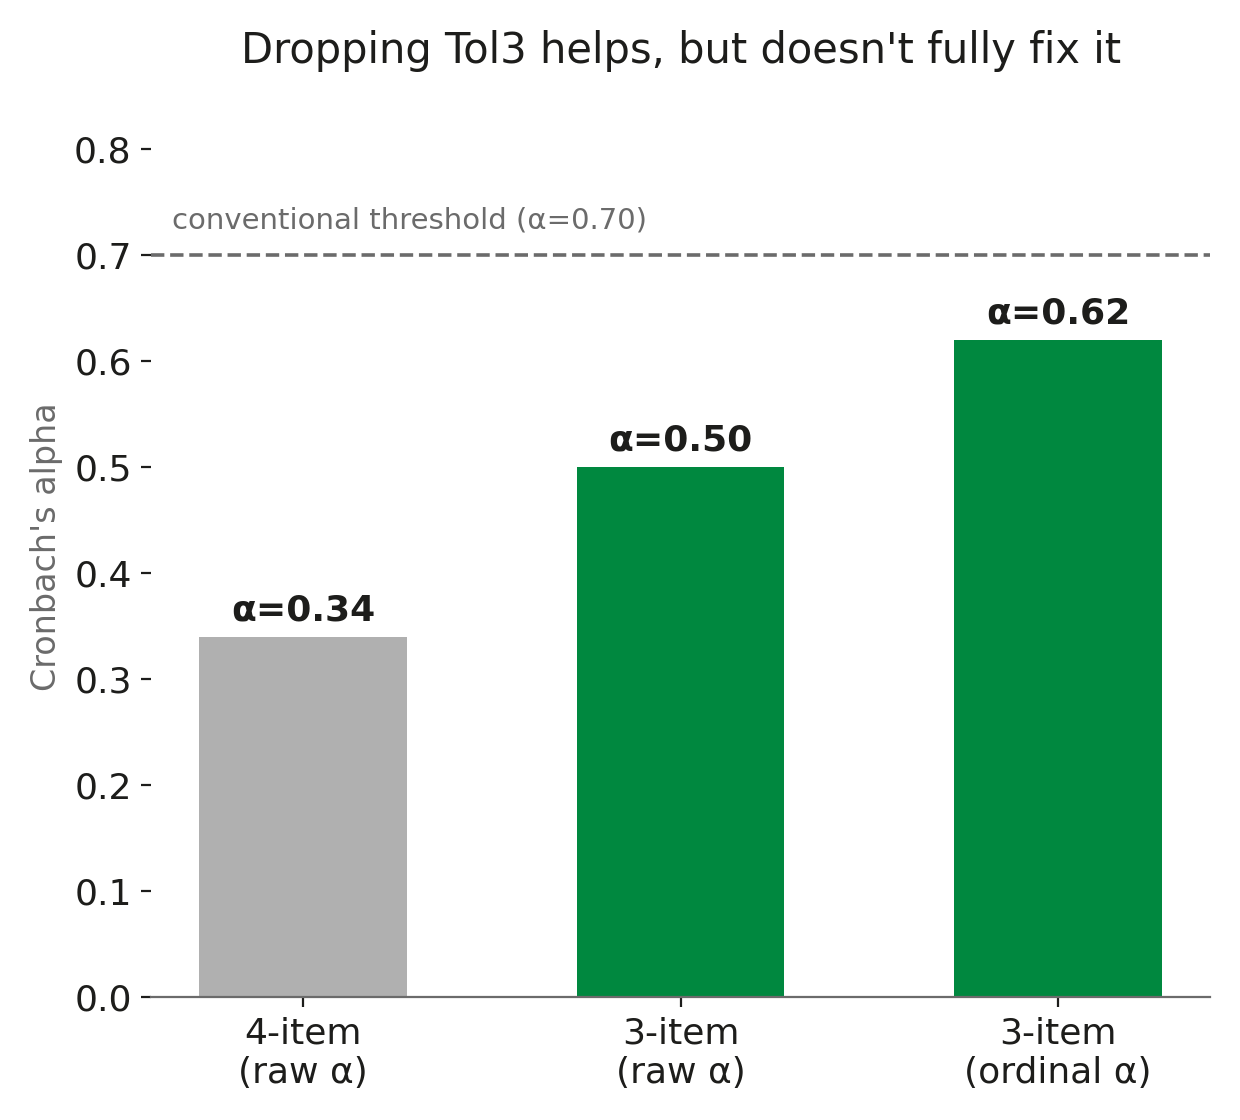
\includegraphics[width=0.75\textwidth]{figures/fig_reliability.png}
\caption{Tolerance scale reliability (Cronbach's $\alpha$): four-item raw,
three-item raw, and three-item ordinal (polychoric), against the
conventional 0.70 threshold.}
\label{fig:reliability}
\end{figure}

\subsection{Formative versus reflective: intangible cost}
\label{measurement:formative}

A second measurement question concerns how intangible cost (IC) -- a
respondent's general evaluative attitude toward wild boar, together with a
spontaneous emotional reaction captured in a three-word description -- should
be modelled: as a \emph{reflective} construct, whose indicators are
interchangeable symptoms of one underlying attitude (as tolerance is treated
above), or as a \emph{formative} construct, whose indicators are distinct
ingredients that combine to define the construct, and need not correlate with
each other at all.

The original questionnaire design specifies intangible cost, alongside
conflict experience, tangible cost, compensation anticipation, and policy
support, as formative by default. We tested this assumption in two ways.
First, EFA on intangible cost's own items shows weak-to-absent common-factor
structure (KMO $= 0.51$; parallel analysis suggests essentially zero
underlying factors) -- the items do not behave like correlated symptoms of one
hidden cause, which is expected and unproblematic for a formative composite,
but would be a problem if IC were meant to be reflective. Second, and more
directly, we forced intangible cost into a reflective specification and
tested its discriminant validity against tolerance using the
heterotrait-monotrait ratio of correlations (HTMT; \citealp{Henseler2015}).
For this test the reflective intangible-cost factor used its two complete
items, the general attitude rating and the first word rating; the second
and third word ratings were left out because many respondents gave fewer
than three words. The result was HTMT $= 1.17$, above the conventional 1.0 ceiling: under a
reflective assumption, the model cannot statistically distinguish intangible
cost's items from tolerance's items at all. This second, more aggressive test
was reserved for intangible cost specifically -- rather than for tangible
cost or the other formative constructs -- because IC's items are the ones
conceptually closest to tolerance itself (an attitude and an emotional
reaction, rather than a physical damage measure), making it the one construct
where a measurement-model mistake could plausibly conflate a predictor with
the outcome it predicts.

Taken together, both checks point the same way: intangible cost is retained
as a formative composite, as originally specified. Its indicators are
ingredients that build the concept, not interchangeable symptoms of it, and
treating it as reflective would have been the wrong measurement choice --
not merely a weaker one.

\subsection{Why tolerance is reflective and intangible cost is formative}
\label{measurement:why-different}

Treating one construct as reflective and another as formative is not an
inconsistency: the choice is made construct by construct, and it is a
conceptual decision about the direction of the relationship between a
construct and its items, not a statistical one. The standard criteria
\citep{Jarvis2003} ask four questions. Does the construct cause the item
responses (reflective), or do the items together make up the construct
(formative)? Are the items interchangeable? Should they correlate with
each other? And does dropping an item change what the construct means?

For tolerance, the Wildlife Tolerance Model \citep{Kansky2016} treats the
items as expressions of one underlying disposition: a more tolerant resident
is expected to support non-lethal management, oppose stricter control, and
accept some damage, all at once. That is the reflective logic, and it is why
we could test it with factor analysis and drop Tol3 without redefining the
construct. For intangible cost, the items are a general attitude rating and
the valence of up to three freely chosen words. The original model specifies
this block, like the other cost and experience blocks, as an index built
from its components, which need not correlate.

We do not want to overstate how clean this distinction is. The empirical
checks are compatible with our choice but do not prove it. Tolerance's
reliability is modest even after dropping Tol3
(Section~\ref{measurement:efa-cfa}), and its three items cover different
content, so a formative reading of tolerance is defensible too. Conversely,
an attitude rating and word valences could reasonably be read as expressions of
one attitude, that is, as reflective. Weak correlations among items do not by themselves make a
construct formative. For this reason we checked whether the choice matters.
Re-estimating the full model with tolerance weighted formatively (PLS mode~B)
instead of reflectively (mode~A) leaves the results unchanged: the
compensation path is $-0.108$ instead of $-0.109$, intangible cost $-0.334$
instead of $-0.338$, intangible benefit $+0.162$ instead of $+0.156$,
prevention effectiveness $+0.107$ instead of $+0.113$, all still
significant, and $R^2$ is $0.235$ instead of $0.234$. The alternative
for intangible cost was tested in Section~\ref{measurement:formative}: as a
reflective construct it cannot be separated from tolerance. Our conclusions
therefore do not depend on the reflective/formative labels, but the closeness
of intangible cost to tolerance is a limitation in either specification
(Section~\ref{discussion:limitations}).

\subsection{Feature engineering}
\label{measurement:features}

Three engineered features feed into the main model. First, as described
above, tolerance enters as the three-item composite Tol1+Tol2+Tol4. Second,
all skewed monetary and area variables (household income, household assets,
economic loss from damage, insurance willingness-to-pay, damaged crop area)
are log(1+x)-transformed. Third, survey site (Baoxing vs.\ Qingchuan) is
engineered as an explicit binary covariate, because Section~\ref{data:confound}
showed that compensation participation is strongly confounded with county;
without this covariate, county differences would be invisible to the model
and could be misattributed to compensation status or conflict experience.

We additionally engineered, but did not use as a control in the primary
model, a household wealth/livelihood index via principal component analysis
(PCA; R package \texttt{factoextra} \citep{Rfactoextra}) on 15 previously-unused variables (crop areas by type, livestock counts
by type, and total land/livestock/asset value). The first principal component
explains 27.9\% of the variance in these 15 variables and correlates strongly
with total household assets ($r = 0.75$) but only weakly with annual cash
income ($r = 0.17$), indicating that income is a poor proxy for asset wealth
in this sample. This index does not predict tolerance directly ($p = .33$),
but it does predict self-reported economic loss strongly
(unstandardised coefficient $0.28$ on log loss, $p < .001$): wealthier households have more agricultural
assets at risk and report more loss accordingly. The original Wildlife
Tolerance Model used a single manifest item (crop asset value) as its only
wealth control; this index shows that a richer, PCA-based wealth measure is
available, though it functions as a socioeconomic control rather than a new
psychological construct, and was therefore not added to the primary
structural model reported in Section~\ref{model}.
